\documentclass[11pt]{beamer}
\usetheme{Copenhagen}
\usepackage[utf8]{inputenc}
\usepackage{amsmath}
\usepackage{amsfonts}
\usepackage{amssymb}
\usepackage{graphicx}
\usepackage[backend=bibtex,style=ieee]{biblatex}
\addbibresource{abe-blockchain.bib}
\author{Andrei Cristian}
\title{Using ABE to Secure Blockchain Transaction Data}
\setbeamercovered{transparent} 
\setbeamertemplate{navigation symbols}{} 
%\logo{} 
%\institute{} 
%\date{} 
%\subject{} 
\begin{document}

\begin{frame}
\titlepage
\end{frame}

\begin{frame}{Table of Contents}
\tableofcontents
\end{frame}

\section{Introduction}
\begin{frame}{Introduction}
\begin{itemize}
	\item Blockchain technology is increasingly being adopted as a trusted platform to support business functions including trusted and verifiable transactions, tracking, and validation.
	\item Most business use-cases require privacy and confidentiality for data and transactions $\Rightarrow$ \textbf{Private blockchain solutions} $\Rightarrow$ Unable to take full advantage of the capabilities, benefits and infrastructure of public blockchain systems.
	\item \textbf{Attribute-Based Encryption} security solution built on private-over-public (PoP) blockchain $\Rightarrow$ Businesses will be able to \textbf{restrict access}, \textbf{maintain privacy}, \textbf{improve performance}, while still being able to benefit from the distributed trust of public blockchains.
\end{itemize}
\end{frame}

\begin{frame}[allowframebreaks]{Public and Private Blockchains}
\begin{itemize}
	\item Similarities\cite{jayachandran}:
	\begin{enumerate}
		\item both are decentralized peer-to-peer networks, where each participant maintains a replica of a shared append-only ledger of digitally signed transactions;
		\item both maintain the replicas in sync through a protocol referred to as consesnsus;
		\item both provide certain guarantees on the immutability of the ledger, even when some participants are faulty or malicious.	
	\end{enumerate}
	\item The main distinction between public and private blockchain is related to who is allowed to participate in the network.
	\item One of the drawbacks of the public blockchain is the substantial amount of computational power to maintain a distributed ledger at a large scale to achieve consensus, in which each node in a network must solve a complex, resource-intensive cryptographic problem - called Proof of Work (PoW)\cite{nakamoto2008} to ensure all are in sync.
	\item Another disadvantage is the openness of public blockchain, which implies little to no privacy protection for transactions and only supports a weak notion of security.
	\item Many people believe private blockchains could provide solutions to many financial enterprise problems, that public blockchains do not, such as abiding by regulations such as Health Insurance Portability and Accountability Act (HIPPA), anti-money laundering (AML) and know-your-customer (KYC) laws, etc.
	\item Private blockchain is usually much faster, cheaper and respects the company's privacy.
	\item  Private blockchains also provide more control power over the participants in the blockchain.
	\item \textbf{Cross-chain} functionality aims to combine the best features of different blockchain systems\cite{liebkind2018}, both private and public, for the purposes of exchanging value across disconnected ecosystems.
	\item None of existing solutions clearly addressed the problem of applying access control policies to enforce data privacy protection on transaction secrets.
	\item For example, when using smart contract solutions, e.g. Ethereum\cite{ethereumweb}, for procurement in supply-chain, transaction parameters such as product name, quantity, price, purchasing terms, shipping options, address, etc. could all be \textbf{sensitive business secrets}. They should be only viewable for relevant stakeholders. 				\item Hyperledger\cite{cachin2016} addresses this problem by relying on a TA approach to build permission groups for data access control. However, data access must be \textbf{predefined} which is not suitable for complex and dynamic businesses logic that require dynamic access control.
	\item \textbf{RBAC} is \textbf{incompatbile} with the distributed nature of blockchain operations where transaction data are mobile and shared by multiple blockchain participants.
\end{itemize}

\end{frame}

\begin{frame}{POP architecture}

\begin{figure}[!ht]
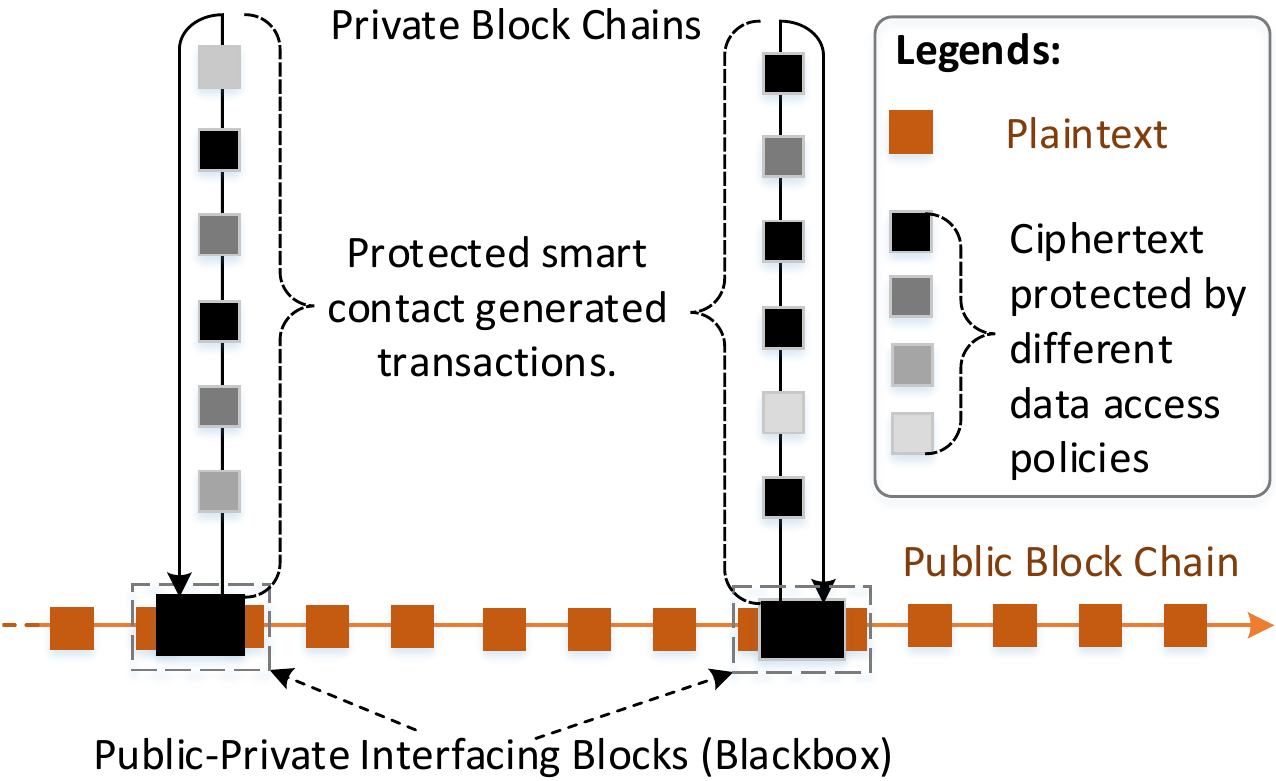
\includegraphics[scale=0.25]{pop.png}
\caption{Illustration of PoP blockchain architecture.}
\label{fig:poparchitecture}
\end{figure}

\end{frame}

\begin{frame}[allowframebreaks]{ABE over PoP Blockchain}
\begin{itemize}
	\item PoP architecture is presented in Figure \ref{fig:poparchitecture}.
	\item Applying ABE on an off-chain basis means it can inter-operate with the public blockchain without interference.
	\item  Private blockchains transactions can be much
\textbf{less computationally intensive} and provide \textbf{superior performance} since they do not have to be verified by all participants.
	\item Businesses are able to choose the private blockchain solution that \textbf{best suits their needs} independently from the public blockchain.
	\item Each private blockchain can be viewed as a \textbf{protected state channel}.
	\item The integrity of a private blockchain can be validated and checked in ciphertext and in aggregate by all public blockchain participants.
	\item The public blockchain infrastructure is leveraged to provide \textbf{validation} and \textbf{immutability} for the entirety of the private blockchain state channel.
	\item This can take
the form of the final private blockchain transaction result, or a hash of the entire private blockchain $\Rightarrow$ distributed trust on the public chain is \textbf{not necessary} for the private blockchain.
	\item \textbf{ABE} provides \textbf{data privacy} for the private blockchain state channel.
	\item Only participants with the appropriate permissions and corresponding ABE attribute private keys can view and validate their relevant blocks in the private block chain.
	\item It provides the benefits of private blockchains in terms of privacy without requiring the deployment of trusted nodes or multiple verification nodes.
	\item It essentially minimizes the entry cost businesses in adopting blockchain solutions.
\end{itemize}
\end{frame}

\begin{frame}[allowframebreaks]{The PoP Solution}
In summary, the presented PoP solution has the following main features:
\begin{itemize}
	\item It is a decentralized trust model for key management of ABE-based data access control. Using this approach, it can incorporate access control policies into ciphertext to protect content of smart contracts.
	\item It is a privacy-preserving messaging protocol to allow private blockchain participants to interact with the smart contract that can generate a private blockchain. This chapter illustrates how to use this protocol based on a supply-chain procurement application.
	\item The solution provides two smart contracts: PPP (Public Parameters and Policies) to establish attribute based security trust model and ppSCM to provide secure data access control based on ABE scheme.
	\item A comprehensive security and performance analysis is presented based on the presented PPP scheme. The presented solution is practical that can significantly reduce the effort and cost to establish dedicated and isolated private blockchains.


\end{itemize}

\end{frame}

\section{System and Models}
\begin{frame}{System and Models}
\begin{itemize}
	\item To illustrate the presented solution, in Figure \ref{fig:supplychain} it is used a supply chain example based on Block-Chain Technology(BCT), which involves multiple parties.
	\item The potential of having all the information written in a blockchain allows the creation of an authoritative record that can be used to automatically establish smart contracts.
	\item Because the information is registered on a
distributed database, it makes it tamper-resistant and fosters greater trust in the trade
network.
\end{itemize}
\end{frame}

\begin{frame}{Supply chain example}
\begin{figure}[!ht]
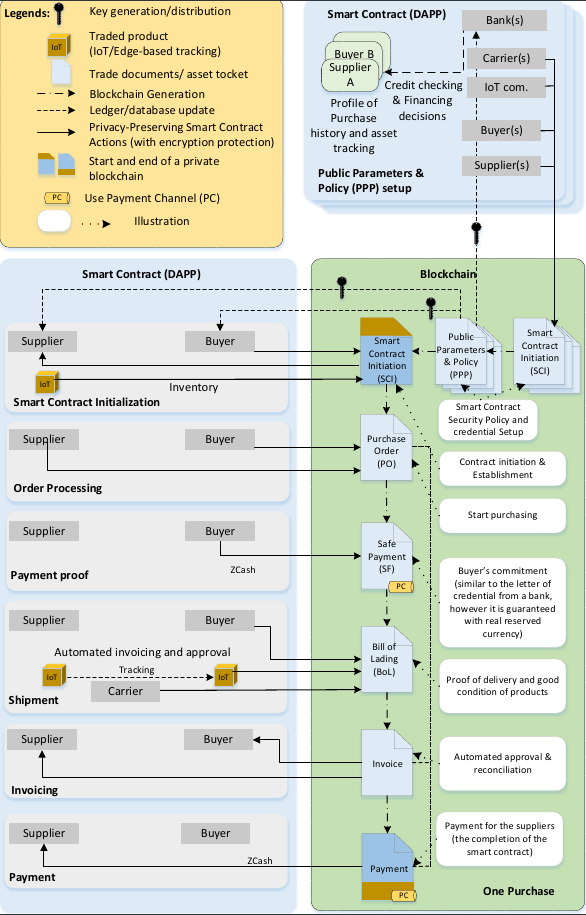
\includegraphics[scale=0.21]{supplychainexample.png}
\caption{A supply chain scenario using IoT devices, blockchain, and data encryption protections.}
\label{fig:supplychain}
\end{figure}
\end{frame}

\begin{frame}{Legends and Smart Contract interaction with Blockchain}
\begin{figure}[!ht]
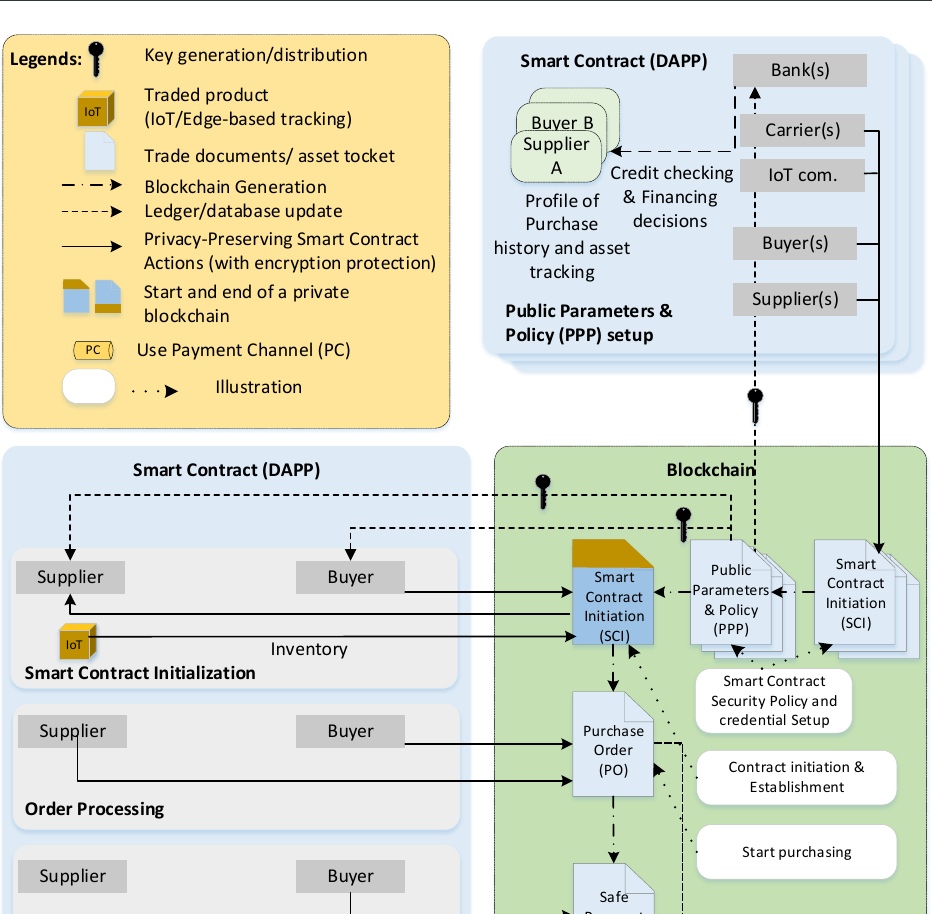
\includegraphics[scale=0.20]{supplychainlegendsscb.png}
\caption{Zoom-in on Legends and interaction of the first smart contract with the blockchain}
\label{fig:supplychainlegendsscb}
\end{figure}
\end{frame}

\begin{frame}{Smart Contract interaction with Blockchain}
\begin{figure}[!ht]
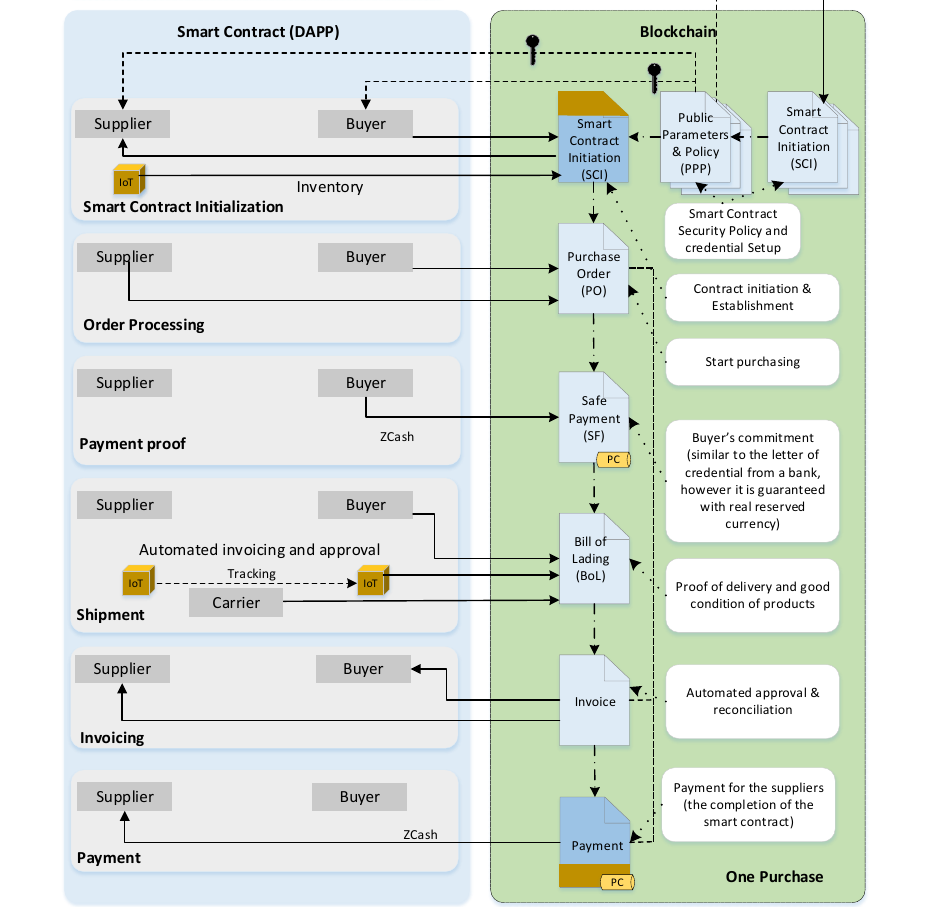
\includegraphics[scale=0.20]{supplychainscb.png}
\caption{Zoom-in on the interaction of the second smart contract with the blockchain}
\label{fig:supplychainscb}
\end{figure}
\end{frame}

\section{PoP System Models}
\begin{frame}{PoP System Models}
\begin{itemize}
	\item PoP System Models
\end{itemize}
\end{frame}

\section{PoP Operation and Performance Analysis}
\begin{frame}{PoP Operation and Performance Analysis}
\begin{itemize}
	\item PoP Operation and Performance Analysis
\end{itemize}
\end{frame}

\section{Summary}
\begin{frame}{Summary}
\begin{itemize}
	\item Summary
\end{itemize}
\end{frame}

\section{References}
\begin{frame}[allowframebreaks]{References}
\printbibliography
\end{frame}

\end{document}